\documentclass[a4paper,twoside]{ociamthesis}
% This one will format for one-sided binding (ie left margin > right margin; no extra blank pages):
%\documentclass[a4paper]{ociamthesis}
% This one will format for PDF output (ie equal margins, no extra blank pages):
%\documentclass[a4paper,nobind]{ociamthesis} 

%%%%% SELECT YOUR DRAFT OPTIONS
% Three options going on here; use in any combination.  But remember to turn the first two off before
% generating a PDF to send to the printer!

% This adds a "DRAFT" footer to every normal page.  (The first page of each chapter is not a "normal" page.)
\fancyfoot[C]{\emph{DRAFT version \today}}  

% This highlights (in blue) corrections marked with (for words) \mccorrect{blah} or (for whole
% paragraphs) \begin{mccorrection} . . . \end{mccorrection}.  This can be useful for sending a PDF of
% your corrected thesis to your examiners for review.  Turn it off, and the blue disappears.
\correctionstrue{}

% Standard packages and definitions
\usepackage{tabularx}
\usepackage{subcaption}
\usepackage{footnote}
\usepackage{lipsum}  
\usepackage[version=4]{mhchem}
\usepackage{float}
\usepackage{bold-extra}
\usepackage{abstract}

\captionsetup{format=hang}
\newcolumntype{C}{>{\centering\arraybackslash}X}
\newcolumntype{L}{>{\raggedright\arraybackslash}X}
\newcolumntype{R}{>{\raggedleft\arraybackslash}X}

% Colors
\preparecolorset{rgb}{}{}{
AliceBlue,.94,.972,1;%
AntiqueWhite,.98,.92,.844;%
Aqua,0,1,1;%
Aquamarine,.498,1,.83;%
Azure,.94,1,1;%
Beige,.96,.96,.864;%
Bisque,1,.894,.77;%
Black,0,0,0;%
BlanchedAlmond,1,.92,.804;%
Blue,0,0,1;%
BlueViolet,.54,.17,.888;%
Brown,.648,.165,.165;%
BurlyWood,.87,.72,.53;%
CadetBlue,.372,.62,.628;%
Chartreuse,.498,1,0;%
Chocolate,.824,.41,.116;%
Coral,1,.498,.312;%
CornflowerBlue,.392,.585,.93;%
Cornsilk,1,.972,.864;%
Crimson,.864,.08,.235;%
Cyan,0,1,1;%
DarkBlue,0,0,.545;%
DarkCyan,0,.545,.545;%
DarkGoldenrod,.72,.525,.044;%
DarkGray,.664,.664,.664;%
DarkGreen,0,.392,0;%
DarkGrey,.664,.664,.664;%
DarkKhaki,.74,.716,.42;%
DarkMagenta,.545,0,.545;%
DarkOliveGreen,.332,.42,.185;%
DarkOrange,1,.55,0;%
DarkOrchid,.6,.196,.8;%
DarkRed,.545,0,0;%
DarkSalmon,.912,.59,.48;%
DarkSeaGreen,.56,.736,.56;%
DarkSlateBlue,.284,.24,.545;%
DarkSlateGray,.185,.31,.31;%
DarkSlateGrey,.185,.31,.31;%
DarkTurquoise,0,.808,.82;%
DarkViolet,.58,0,.828;%
DeepPink,1,.08,.576;%
DeepSkyBlue,0,.75,1;%
DimGray,.41,.41,.41;%
DimGrey,.41,.41,.41;%
DodgerBlue,.116,.565,1;%
FireBrick,.698,.132,.132;%
FloralWhite,1,.98,.94;%
ForestGreen,.132,.545,.132;%
Fuchsia,1,0,1;%
Gainsboro,.864,.864,.864;%
GhostWhite,.972,.972,1;%
Gold,1,.844,0;%
Goldenrod,.855,.648,.125;%
Gray,.5,.5,.5;%
Green,0,.5,0;%
GreenYellow,.68,1,.185;%
Grey,.5,.5,.5;%
Honeydew,.94,1,.94;%
HotPink,1,.41,.705;%
IndianRed,.804,.36,.36;%
Indigo,.294,0,.51;%
Ivory,1,1,.94;%
Khaki,.94,.9,.55;%
Lavender,.9,.9,.98;%
LavenderBlush,1,.94,.96;%
LawnGreen,.488,.99,0;%
LemonChiffon,1,.98,.804;%
LightBlue,.68,.848,.9;%
LightCoral,.94,.5,.5;%
LightCyan,.88,1,1;%
LightGoldenrod,.933,.867,.51;%
LightGoldenrodYellow,.98,.98,.824;%
LightGray,.828,.828,.828;%
LightGreen,.565,.932,.565;%
LightGrey,.828,.828,.828;%
LightPink,1,.712,.756;%
LightSalmon,1,.628,.48;%
LightSeaGreen,.125,.698,.668;%
LightSkyBlue,.53,.808,.98;%
LightSlateBlue,.518,.44,1;%
LightSlateGray,.468,.532,.6;%
LightSlateGrey,.468,.532,.6;%
LightSteelBlue,.69,.77,.87;%
LightYellow,1,1,.88;%
Lime,0,1,0;%
LimeGreen,.196,.804,.196;%
Linen,.98,.94,.9;%
Magenta,1,0,1;%
Maroon,.5,0,0;%
MediumAquamarine,.4,.804,.668;%
MediumBlue,0,0,.804;%
MediumOrchid,.73,.332,.828;%
MediumPurple,.576,.44,.86;%
MediumSeaGreen,.235,.7,.444;%
MediumSlateBlue,.484,.408,.932;%
MediumSpringGreen,0,.98,.604;%
MediumTurquoise,.284,.82,.8;%
MediumVioletRed,.78,.084,.52;%
MidnightBlue,.098,.098,.44;%
MintCream,.96,1,.98;%
MistyRose,1,.894,.884;%
Moccasin,1,.894,.71;%
NavajoWhite,1,.87,.68;%
Navy,0,0,.5;%
NavyBlue,0,0,.5;%
OldLace,.992,.96,.9;%
Olive,.5,.5,0;%
OliveDrab,.42,.556,.136;%
Orange,1,.648,0;%
OrangeRed,1,.27,0;%
Orchid,.855,.44,.84;%
PaleGoldenrod,.932,.91,.668;%
PaleGreen,.596,.985,.596;%
PaleTurquoise,.688,.932,.932;%
PaleVioletRed,.86,.44,.576;%
PapayaWhip,1,.936,.835;%
PeachPuff,1,.855,.725;%
Peru,.804,.52,.248;%
Pink,1,.752,.796;%
Plum,.868,.628,.868;%
PowderBlue,.69,.88,.9;%
Purple,.5,0,.5;%
Red,1,0,0;%
RosyBrown,.736,.56,.56;%
RoyalBlue,.255,.41,.884;%
SaddleBrown,.545,.27,.075;%
Salmon,.98,.5,.448;%
SandyBrown,.956,.644,.376;%
SeaGreen,.18,.545,.34;%
Seashell,1,.96,.932;%
Sienna,.628,.32,.176;%
Silver,.752,.752,.752;%
SkyBlue,.53,.808,.92;%
SlateBlue,.415,.352,.804;%
SlateGray,.44,.5,.565;%
SlateGrey,.44,.5,.565;%
Snow,1,.98,.98;%
SpringGreen,0,1,.498;%
SteelBlue,.275,.51,.705;%
Tan,.824,.705,.55;%
Teal,0,.5,.5;%
Thistle,.848,.75,.848;%
Tomato,1,.39,.28;%
Turquoise,.25,.88,.815;%
Violet,.932,.51,.932;%
VioletRed,.816,.125,.565;%
Wheat,.96,.87,.7;%
White,1,1,1;%
WhiteSmoke,.96,.96,.96;%
Yellow,1,1,0;%
YellowGreen,.604,.804,.196}


%%%%% BIBLIOGRAPHY SETUP
\usepackage[
	style=ieee,
	sortcites=false,
	backend=biber,
	doi=true,
	isbn=true,
	maxcitenames=2,
	mincitenames=1,
	uniquelist=true,
	abbreviate,
	maxbibnames=99,
	citestyle=numeric-comp, % Multiple citations delimited by ", "
	% autocite=superscript
]{biblatex}

% Bold authors in bibliography
\DeclareNameWrapperFormat{sortname}{\mkbibbold{#1}}
\DeclareNameWrapperAlias{author}{sortname}
\DeclareNameWrapperAlias{editor}{sortname}
\DeclareNameWrapperAlias{translator}{sortname}
% \renewcommand\citepunct{, } 

% Pretty references
\usepackage[
    pdfpagelabels,
	    colorlinks=true,
    citecolor=blue,
    urlcolor=blue,
    linkcolor=black
]{hyperref} 

\usepackage{bookmark}
	% for linking between references, figures, TOC, etc in the pdf document

% Equation spacing
\expandafter\def\expandafter\normalsize\expandafter{%
    \normalsize%
    \setlength\abovedisplayskip{12pt plus 4pt minus 6pt}%
    \setlength\belowdisplayskip{12pt plus 4pt minus 8pt}%
    % \setlength\abovedisplayshortskip{0pt}%
    % \setlength\belowdisplayshortskip{0pt}%
}

% Change this to the name of your .bib file (usually exported from a citation manager like Zotero or EndNote).
\addbibresource{ref.bib}

\newcommand*{\bibtitle}{References}

% Pages shouldn't have numbering here
\pagenumbering{gobble} 

% Uncomment this if you want equation numbers per section (2.3.12), instead of per chapter (2.18):
%\numberwithin{equation}{subsection}

%%%%% THESIS / TITLE PAGE INFORMATION
% Everybody needs to complete the following:
\title{Suitable Impressive Thesis Title}
\author{John Doe}
\college{Institute of Philology}
\degree{Dr.~rer. nat.}
\degreedate{}


%%%%% YOUR OWN PERSONAL MACROS
% This is a good place to dump your own LaTeX macros as they come up.
\newcommand{\er}[1]{Eq.~\eqref{eq:#1}}
\newcommand{\erp}[2]{Eqns.~\eqref{eq:#1}\eqref{eq:#2}}
\newcommand{\be}[1]{\textsubscript{#1}}  % easier textsubscripts
\newcommand{\ab}[1]{\textsubscript{#1}}  % easier textsubscripts
\renewcommand{\th}{\textsuperscript{th}} % ex: I won 4\th place
\newcommand{\nd}{\textsuperscript{nd}}
\renewcommand{\st}{\textsuperscript{st}}
\newcommand{\rd}{\textsuperscript{rd}}
\newcommand{\vecc}[1]{\mathbf{#1}}
\newcommand{\partialdifof}[2]{\frac{\partial #1}{\partial #2}}
\newcommand{\bt}[1]{\texttt{\textbf{#1}}}

% Custom defs
\newcommand{\isp}{$I_{\mathrm{sp}}$}
\newcommand{\ispm}{I_{\mathrm{sp}}}

\setlength{\jot}{10pt}
\usepackage{xltabular}
\newcolumntype{R}{>{\raggedleft\arraybackslash}X}



\usepackage{fontspec}
\usepackage{unicode-math}
\setmainfont[Scale=0.93]{TeX Gyre Schola}
\setmathfont[Scale=0.93]{TeX Gyre Schola Math}

%%%%% THE ACTUAL DOCUMENT STARTS HERE
\begin{document}

%%%%% CHOOSE YOUR LINE SPACING HERE
% This is the official option.  Use it for your submission copy and library copy:
% \setlength{\textbaselineskip}{16pt plus2pt}
\setlength{\textbaselineskip}{18pt plus1pt minus1pt}
% This is closer spacing (about 1.5-spaced) that you might prefer for your personal copies:
%\setlength{\textbaselineskip}{18pt plus2pt minus1pt}

% You can set the spacing here for the roman-numbered pages (acknowledgements, table of contents, etc.)
\setlength{\frontmatterbaselineskip}{17pt plus1pt minus1pt}

% Leave this line alone; it gets things started for the real document.
\setlength{\baselineskip}{\textbaselineskip}

%%%%% CHOOSE YOUR SECTION NUMBERING DEPTH HERE
% You have two choices.  First, how far down are sections numbered?  (Below that, they're named but
% don't get numbers.)  Second, what level of section appears in the table of contents?  These don't have
% to match: you can have numbered sections that don't show up in the ToC, or unnumbered sections that
% do.  Throughout, 0 = chapter; 1 = section; 2 = subsection; 3 = subsubsection, 4 = paragraph...

% The level that gets a number:
\setcounter{secnumdepth}{2}
% The level that shows up in the ToC:
\setcounter{tocdepth}{2}

% JEM: Pages are roman numbered from here, though page numbers are invisible until ToC.  This is in
% keeping with most typesetting conventions.

% Title page is created here
\maketitle

%%%%% DEDICATION -- If you'd like one, un-comment the following.
%\begin{dedication}
%This thesis is dedicated to\\
%someone\\
%for some special reason\\
%\end{dedication}

%%%%% ACKNOWLEDGEMENTS -- Nothing to do here except comment out if you don't want it.
\begin{acknowledgements}
 	\lipsum[1]
\end{acknowledgements}

\newpage \ \newpage

%%%%% ABSTRACT -- Nothing to do here except comment out if you don't want it.
\renewcommand{\abstractname}{Kurzfassung}
\begin{abstract}
	Dies ist ein deutscher Abstrakt.
\end{abstract}
\newpage \ \newpage
\renewcommand{\abstractname}{Abstract}
\begin{abstract}
    \lipsum[2]
\end{abstract}
\newpage \ \newpage

\dominitoc % include a mini table of contents

% This aligns the bottom of the text of each page.  It generally makes things look better.
\flushbottom

\pagenumbering{roman}

% This is where the whole-document ToC appears:
\tableofcontents

% List of Symbols
\chapter*{List of Symbols}
\mtcaddchapter[List of Symbols]

\begin{center}
\begin{tabular}{cll}

	\textbf{Symbol} & \textbf{Description} & \textbf{Unit}  \\
	\(\vecc{a}\) & acceleration & \si{\metre\per\second\squared}  \\
	\(\vecc{F}\) & force & \si{\newton}  \\
	\(\dot{m}\) & mass-flow & \si{\kilogram\per\second}  \\
	\(\vecc{x}\) & position & \si{m}  \\

\end{tabular}
\end{center}


% List of Abbreviations
\chapter*{List of Abbreviations}
\mtcaddchapter[List of Abbreviations]

\begin{center}
\begin{tabular}{ll}

	\textbf{Abbr.} & \textbf{Description} \\
	AIREBO & Adaptive intermolecular reactive bond order \\
	CEX    & Charge exchange \\
	CP     & Chemical propulsion \\

\end{tabular}
\end{center}


\listoffigures
\mtcaddchapter
% \mtcaddchapter is needed when adding a non-chapter (but chapter-like) entity to avoid confusing minitoc

% Uncomment to generate a list of tables:
%\listoftables
%	\mtcaddchapter

%%%%% CHAPTERS
% Add or remove any chapters you'd like here, by file name (excluding '.tex'):
\flushbottom

\begin{savequote}[8cm]
  Starting from Day 0 became my friend.
  
  \qauthor{--- D. Goggins}
\end{savequote}

\chapter{\label{ch:introduction}Introduction}
\pagenumbering{arabic}

\minitoc

\lipsum[3]

\begin{equation}\label{eq:thrust}
T = \dot{m} u_e
\end{equation}

\begin{figure}[t!]
  \centering
  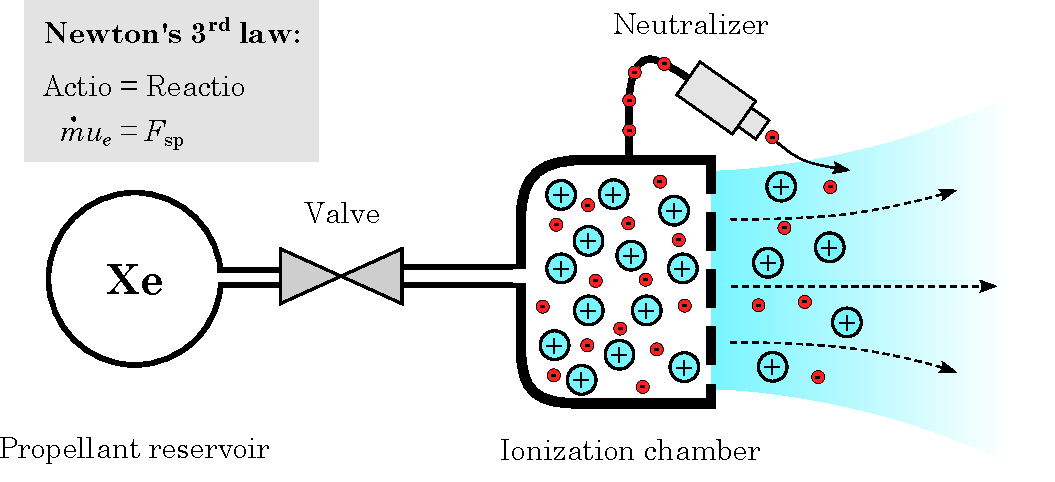
\includegraphics[width=\textwidth]{fig/1.introduction/final/ep_schematic.pdf}
  \caption{Schematic of an electrostatic propulsion device.}
  \label{fig:ep_schematic}
\end{figure}

A schematic of the working principle of an electrostatic thruster is
illustrated in Figure~\ref{fig:ep_schematic}. 

\section{Background and Motivation}\label{sec:background-and-motivation}

The lifetime of most EP devices is limited by erosion becoming so
severe, that the accelerating mechanism does not work properly anymore.

\section{Literature Review}\label{sec:literature-review}

Because there is limited literature available on MD simulations of EP plasma
sputtering according to~\textcite{jackson2019}, this literature review includes
publications from various fields where similar analyses were
conducted~\autocite{harvey2007}.

\begin{savequote}[8cm]
  Keep your eyes on the stars, but remember to keep your feet on the ground.
  
  \qauthor{--- T. Roosevelt}
\end{savequote}

\chapter{\label{ch:theory-of-sputtering}Theory of ion beam sputtering}

\minitoc


Surfaces subjected to ion irradiation undergo a cascade of energetic
displacement on the atomic scale.

\section{Test section}\label{sec:test-section}

%% APPENDICES %% 
% Starts lettered appendices, adds a heading in table of contents, and adds a
%    page that just says "Appendices" to signal the end of your main text.
% \startappendices
% % Add or remove any appendices you'd like here:
% \include{text/appendix-1}


% %%%%% REFERENCES
\printbibliography


\end{document}
